\section{Sample Acronyms}
\label{s:Acronyms}

This is an acronym: \acs{TEST}.

\section{Sample Listings}
\label{s:Listings}

\begin{listing}
\begin{minted}{asm}
; Prologue
mov    [RSP + 8], RCX
push   R15
push   R14
push   R13
mov    RAX,  fixed-allocation-size
call   __chkstk
sub    RSP, RAX
lea    R13, 128[RSP]

; Body
...

; Epilogue
add      RSP, fixed-allocation-size
pop      R13
pop      R14
pop      R15
ret
\end{minted}
\caption{Structure of a function at assembly level \cite{microsoft_corp_x64_2021}}
\label{listing:prolog-epilogl}
\end{listing}

\newpage

\section{Sample Figures}
\label{s:Figures}

\begin{figure}[ht]
\centering
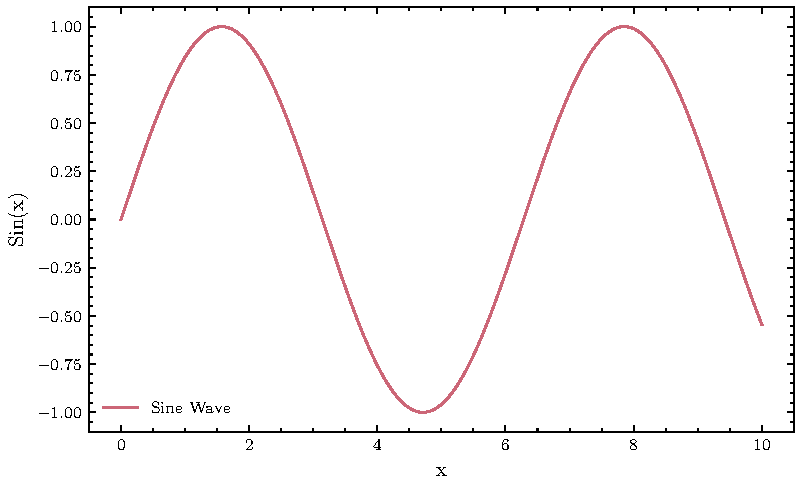
\includegraphics[width=\textwidth,height=\textheight,keepaspectratio]{Python_plotting_example/example_1.pdf}
\caption{Example Flow}
\end{figure}


\newpage

\section{Sample Tables}
\label{s:Tables}

\begin{longtable}[]{@{}
  >{\raggedright\arraybackslash}p{(\columnwidth - 10\tabcolsep) * \real{0.1667}}
  >{\raggedright\arraybackslash}p{(\columnwidth - 10\tabcolsep) * \real{0.1667}}
  >{\raggedright\arraybackslash}p{(\columnwidth - 10\tabcolsep) * \real{0.1667}}
  >{\raggedright\arraybackslash}p{(\columnwidth - 10\tabcolsep) * \real{0.1667}}
  >{\raggedright\arraybackslash}p{(\columnwidth - 10\tabcolsep) * \real{0.1667}}
  >{\raggedright\arraybackslash}p{(\columnwidth - 10\tabcolsep) * \real{0.1667}}@{}}
\toprule()
\begin{minipage}[b]{\linewidth}\raggedright
Technique
\end{minipage} & \begin{minipage}[b]{\linewidth}\raggedright
Do this
\end{minipage} & \begin{minipage}[b]{\linewidth}\raggedright
Do that
\end{minipage} & \begin{minipage}[b]{\linewidth}\raggedright
Do the other
\end{minipage} & \begin{minipage}[b]{\linewidth}\raggedright
Don't do this
\end{minipage} & \begin{minipage}[b]{\linewidth}\raggedright
Don't do that
\end{minipage} \\
\midrule()
\endhead
Sample1 & Sample1 & Sample1 & Sample1 & Sample1 & Sample1 \\
Sample2 & Sample2 & Sample2 & Sample2 & Sample2 & Sample2 \\
\bottomrule()
\caption{Comparison between Sample1 and Sample2}
  \label{t:samples-comparison}
\end{longtable}

\newpage

\section{Sample Algorithms}
\label{s:Algorithms}

\begin{algorithm}[H]
\DontPrintSemicolon
\SetAlgoLined
\KwResult{True if all variables in $b$ are initialized before use}
\SetKwInOut{Input}{Input}\SetKwInOut{Output}{Output}
\Input{b: Block of code}
\Output{status: Integer}
\BlankLine
\setcounter{AlgoLine}{0}

\ForEach{statement $s$ in $b$}{
    \uIf{$s$ is an assignment}{
        mark variable on LHS of $s$ as initialized\;
    }
    \uElseIf{$s$ is a usage of variable $v$}{
        \If{$v$ is not marked as initialized}{
            return UNINITIALIZED\_VARIABLE\_DETECTED\;
        }
    }
    \Else{
        continue\;
    }
}

return NO\_ISSUES\_DETECTED;

\caption{Static check for uninitialized variable usage}
\end{algorithm}
